\documentclass[sigconf,review,anonymous]{acmart}

\usepackage{booktabs}
\usepackage{graphicx}
\usepackage{microtype}
\usepackage{xspace}

\newcommand{\system}{TensorJoin\xspace}

\setcopyright{none}
\settopmatter{printacmref=false,printccs=false,printfolios=true}
\acmConference[Under review]{Anonymous submission}{2026}{}
\acmYear{2026}
\acmDOI{}
\acmISBN{}

\begin{document}

\title[TensorJoin: Certified Precision Routing for Exact GPU Joins]{TensorJoin: Certified Precision Routing\texorpdfstring{\\}{ }for Exact GPU Similarity Joins}

\author{Anonymous Author(s)}
\affiliation{%
  \institution{Anonymous Institution}
  \country{Anonymous}}

\begin{abstract}
Exact high-dimensional similarity joins are expensive on GPUs because a fixed
arithmetic path either spends high precision on easy pairs or risks changing
threshold decisions.  Existing Tensor-Core join implementations improve dense
distance throughput, but their low-precision variants are approximate, while
exact GPU systems retain a full-precision comparison path.  We observe that
precision can instead be treated as an output-sensitive query-planning
decision: a conservative interval around a low-precision score can accept or
reject most pairs, leaving only a small boundary population for more precise
evaluation.  Based on this observation, we present \system, a three-stage
INT8-Tensor-Core/FP32/FP64 router with generated-code-aware numerical
certificates, dynamic compaction, ragged-dimension support, and exact output
reconstruction.  On three public $N=4096$ anchors spanning 128--784
dimensions, the audited dynamic router is $1.271\times$--$2.329\times$ faster
than refining every first-stage ambiguity in FP64.  In a separate scalable
implementation evaluated from pageable FP32 input through sorted host output,
\system returns exactly 3,926,078 directed pairs on a public 60K-vector
self-join and is $5.083\times$ faster than MiSTIC and $11.783\times$ faster
than GDS-Join.  A faster mixed-precision point is not exact, producing 598
false negatives and 1,130 false positives.  We report the audited-router and
full-scale-system results as separate implementation scopes and preserve a
failed same-artifact performance bridge rather than using it to overstate the
evidence.
\end{abstract}

\ccsdesc[500]{Information systems~Similarity measures}
\ccsdesc[300]{Computing methodologies~Massively parallel algorithms}
\keywords{exact similarity join, GPU databases, Tensor Cores, mixed precision, numerical certificates}

\maketitle

\section{Introduction}

A similarity join reports all pairs of vectors whose distance is at most a
threshold.  It is a basic primitive for duplicate detection, clustering,
graph construction, and vector-data analysis.  Unlike approximate nearest
neighbor search, an exact join cannot silently lose a pair close to the
decision boundary.  This output contract makes high-dimensional GPU execution
awkward: dense low-precision matrix multiplication is fast, but the final
Boolean predicate is sensitive to small numerical errors; evaluating every
pair in high precision preserves the contract but ignores the much higher
throughput of modern matrix units.

Exact GPU join systems use spatial or metric organization
~\cite{gowanlock2019gpuselfjoin,donnelly2024mistic}.  Separately, Tensor-Core
methods accelerate dense similarity computations with reduced or mixed
precision~\cite{ahle2020tensorcore,gallet2022distance,curless2025fasted}.
These approaches leave a gap.  A global high-precision choice wastes work on
pairs that lie far from the radius, whereas a global low-precision choice may
change the output set.  Approximate candidate generation followed by exact
refinement is common in vector search, but candidate refinement alone does not
certify the pairs discarded by the approximate stage.

Our key observation is that arithmetic precision can be a per-pair query-plan
decision.  For each quantized vector, \system retains a residual-error bound.
The low-precision distance and the two residual bounds define an interval that
contains the exact distance.  An interval wholly below the threshold safely
accepts the pair; one wholly above safely rejects it; and only an interval that
crosses the threshold advances.  The query plan therefore routes uncertainty,
not all input pairs, through progressively more expensive precision stages.

Turning this idea into a GPU operator requires more than an algebraic bound.
The implementation must account for the arithmetic actually emitted by the
compiler, compact uncertain pairs without corrupting output order, launch later
stages over measured rather than allocated extents, support dimensions that do
not align with matrix-multiply tiles, and reconstruct a canonical exact result.
\system addresses these requirements with an INT8 Tensor-Core front end, a
certified FP32 filter, exact FP64 refinement, and explicit count-read edges
between stages.  Figure~\ref{fig:teaser} summarizes the resulting precision
funnel and the separately scoped full-scale comparison.

\begin{figure*}[t]
  \centering
  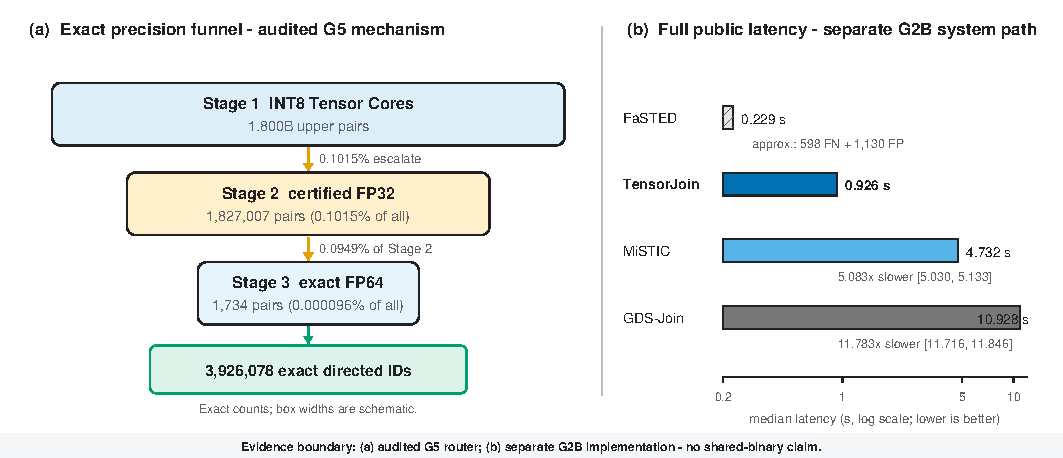
\includegraphics[width=\textwidth]{figures/fig1_evidence_separated_teaser.pdf}
  \Description{Two-panel teaser.  The left panel shows the measured pair
  population shrinking through INT8, FP32, and FP64 stages.  The right panel
  compares full public-denominator latency and distinguishes three exact
  systems from an approximate FaSTED point.}
  \caption{Certified routing concentrates high precision on the decision
  boundary, while a separately scoped scalable implementation establishes
  external-system impact.  In the exact G5 full-scale mechanism run, only
  0.1015\% of 1.800B upper pairs advance from INT8 Tensor Cores to certified
  FP32, and 1,734 pairs advance to exact FP64 before reconstruction of
  3,926,078 directed IDs.  Under the separate G2B
  pageable-host-input-to-sorted-host-output contract, \system has a 0.926~s
  median and is $5.083\times$ and $11.783\times$ faster than exact MiSTIC and
  GDS-Join, respectively; the 0.229~s FaSTED point has 598 false negatives and
  1,130 false positives.  Panels (a) and (b) use different frozen
  implementation scopes and do not constitute a shared-binary claim.}
  \label{fig:teaser}
\end{figure*}

This paper makes three contributions:
\begin{itemize}
  \item We formulate exact threshold evaluation as a three-stage precision
  certificate that converts low-precision matrix-unit scores into safe
  accept, reject, or refine decisions.  The implementation is checked against
  an independent FP64 oracle, adversarial transformations, selected generated
  code, memory sanitization, and sustained stress.
  \item We realize the certificate as an output-sensitive GPU query plan with
  compaction, actual dynamic launch extents, and ragged-dimension support.  On
  public SIFT (128-D), CIFAR-GIST (512-D), and Fashion-MNIST (784-D) anchors,
  this router
  improves over an otherwise identical path that sends every first-stage
  ambiguity to FP64 by $1.271\times$, $2.329\times$, and $1.710\times$.
  \item We evaluate a scalable exact implementation against external GPU join
  systems under a complete public 60K self-join denominator.  It reproduces
  the exact output and is $5.083\times$ faster than the strongest exact
  external comparator.  We also expose, rather than hide, the quality gap of
  the faster approximate point and the variability that prevented a
  same-artifact performance unification claim.
\end{itemize}

\section{Problem and Contract}

Let $X=\{x_0,\ldots,x_{N-1}\}$ be vectors in $\mathbb{R}^{D}$ and let
$\varepsilon$ be a radius.  The self-join emits
\begin{equation}
  J(X,\varepsilon)=\{(i,j):\lVert x_i-x_j\rVert_2^2\leq\varepsilon^2\}.
\end{equation}
We require exact equality with an FP64 distance oracle evaluated over the
stored FP32 vectors.  The output is represented as sorted canonical 64-bit
pair identifiers.  Self pairs are retained and accepted upper-triangular
off-diagonal pairs are mirrored during reconstruction.

This definition separates three properties that are often conflated.
Candidate recall states whether a first pass preserves every true pair;
distance accuracy bounds a numerical approximation; exact join semantics
requires that the final emitted set match the oracle, including at the
threshold.  \system targets the third property.  It may use approximate
arithmetic internally only when a certificate proves the associated decision
safe or when the pair is passed to a more precise stage.

Our public system denominator begins with a pageable-host FP32 array and ends
with sorted host-resident 64-bit identifiers.  It includes quantization,
analytic residual construction, allocations, host-to-device movement, all
dynamic GPU stages and count reads, device-to-host accepted-ID copies,
symmetrization, concatenation, and sorting.  File I/O, process startup, CUDA
context creation, compilation, validation hashes, and optional pair-file
serialization are outside the timer.  The mechanism attribution experiment
uses a narrower resident-input/output operator denominator and is labeled as
such throughout the paper.

\section{Certified Precision Routing}

\subsection{INT8 interval certificate}

For each FP32 vector $x$, symmetric per-vector quantization produces a signed
INT8 code $z_x$, a scale $s_x$, and reconstruction
$\widehat{x}=s_xz_x$.  The preprocessing step also stores a conservative
residual norm $e_x\geq\lVert x-\widehat{x}\rVert_2$.  For two vectors $q$ and
$x$, an INT8/INT32 matrix multiply supplies the dot-product term of
$\widehat d=\lVert\widehat q-\widehat x\rVert_2$.  The triangle inequality
then gives
\begin{align}
  L_1(q,x) &= \max(0,\widehat d-e_q-e_x)^2,\\
  U_1(q,x) &= (\widehat d+e_q+e_x)^2,
\end{align}
with $L_1\leq\lVert q-x\rVert_2^2\leq U_1$ after the declared outward
implementation guard.  If $U_1\leq\varepsilon^2$, the pair is accepted.  If
$L_1>\varepsilon^2$, it is rejected.  Otherwise its identifier is appended to
the stage-1 ambiguity buffer.

The mathematical inequality is not by itself a machine-level proof.  The
SM120 implementation uses an accumulator range for which INT32 accumulation
cannot overflow and integer-to-FP32 conversion remains exact for the tested
dimensions.  Its final interval includes conservative margins for the emitted
FP32 instruction sequence, approximate square root, and flush-to-zero
behavior.  We audit the runtime-selected function rather than inferring the
machine operations from source alone.

\subsection{Certified FP32 boundary filter}

The middle stage loads only compacted stage-1 ambiguities and computes an FP32
squared distance.  A reduction-order-independent error envelope, augmented by
implementation padding for the emitted reduction and final expression,
produces $[L_2,U_2]$.  It applies the same three-way rule: accept when
$U_2\leq\varepsilon^2$, reject when $L_2>\varepsilon^2$, and compact only the
remaining pairs for FP64.

The scale of the guard matters.  An early version used a unit-floor term and
became unnecessarily loose under a $2^{-8}$ metamorphic scaling test.  The
admitted implementation instead scales its expression margin with the
distance magnitude while retaining explicit absolute terms for the
flush-to-zero floor.  This negative result is useful: a safe but poorly scaled
bound can preserve correctness while destroying the output-sensitive behavior
the query plan depends on.

\subsection{Exact FP64 fallback}

The final stage evaluates the original stored FP32 vectors in FP64 and applies
the join predicate directly.  FP64 is therefore the semantic backstop, not an
unverified estimate.  On the full-scale precision-funnel run, stage 1 leaves
1,827,007 of 1,800,030,000 upper-triangular pairs unresolved.  Stage 2 accepts
713,664 and rejects 1,111,609 of them, leaving only 1,734 FP64 evaluations:
871 accepts and 863 rejects.

\section{GPU Query Plan}

Figure~\ref{fig:pipeline} shows the complete execution graph.  \system tiles
the upper triangle into $64\times64$ output blocks and uses a $K$ step of 64.
For the 60,000-by-512 workload, this produces 440,391 scheduled tiles.  The
runner processes 4,096 tiles per batch, for 108 batches, so temporary pair-ID
buffers remain bounded while the matrix-unit stage stays regular.

\begin{figure*}[t]
  \centering
  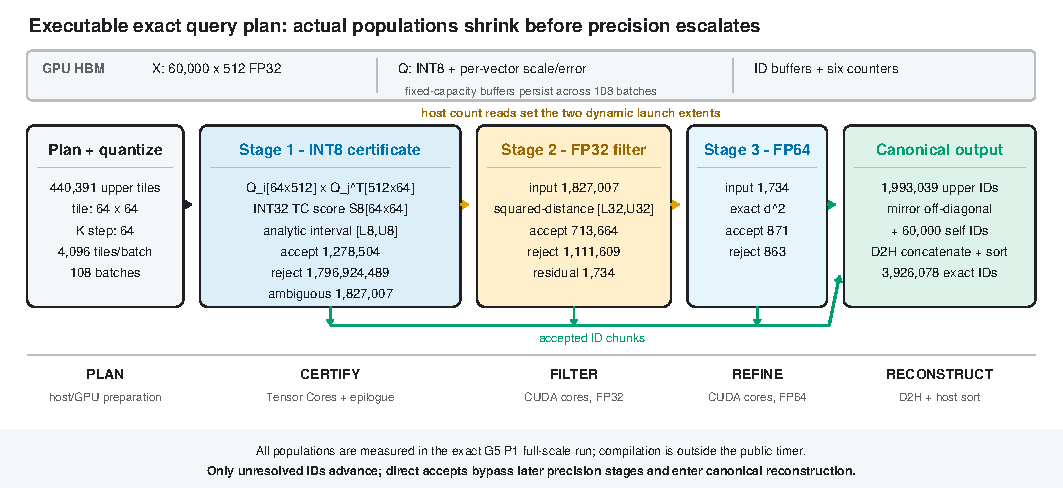
\includegraphics[width=\textwidth]{figures/fig2_exact_precision_routing_pipeline.pdf}
  \Description{A left-to-right exact query plan.  Plan and quantization feed an
  INT8 Tensor-Core certificate, dynamically compacted uncertain pairs advance
  through certified FP32 and exact FP64, and accepted upper-triangular IDs are
  reconstructed into a sorted directed output.}
  \caption{\system executes precision escalation as a dynamic exact query
  plan.  The full-scale G5 implementation quantizes 60,000-by-512 FP32
  vectors, schedules 440,391 upper $64\times64$ tiles in 108 batches,
  classifies each INT8 Tensor-Core score with an analytic interval, and reads
  actual ambiguous counts before launching certified FP32 and exact FP64 work.
  Direct accepts bypass later stages and join the accepted-ID path; host
  reconstruction mirrors off-diagonal pairs, retains self pairs, concatenates
  IDs, and sorts the final 3,926,078-entry canonical output.  Compilation is
  outside the depicted public timing scope.}
  \label{fig:pipeline}
\end{figure*}

\subsection{Dynamic work rather than capacity work}

Each stage writes accepted or unresolved identifiers and increments a separate
counter.  A host count read is an explicit readiness edge: stage 2 is launched
over the measured stage-1 ambiguity, and stage 3 is launched over the measured
stage-2 remainder.  The implementation never substitutes buffer capacity for
actual population.  This distinction is central when only a small fraction of
pairs lies near the threshold; a nominally selective filter that still
launches the next stage over capacity would not realize an output-sensitive
query plan.

The price of dynamic routing is visible and charged.  It includes compaction
atomics, counter synchronization, dispatch, accepted-ID movement, and final
reconstruction.  Later stages use one program per compacted pair.  Stage 1
uses one independent cooperative thread array per tile; no inter-block barrier
or shared ownership is required.

\subsection{Ragged dimensions and exact reconstruction}

The matrix path pads or masks the final reduction step for dimensions that are
not multiples of the tile width.  This is required for the 784-dimensional
Fashion-MNIST anchor and prevents padded lanes from altering either the score
or its certificate.  The accepted upper-triangular identifiers from every
stage are copied to the host, concatenated, mirrored for off-diagonal pairs,
combined with self pairs, and sorted.  Buffer-overflow checks, duplicate
checks, ID-range checks, and equality with the independent oracle are part of
the validation contract.

\section{Evaluation}

We ask four questions: (1) Does \system return the exact output? (2) Does
dynamic precision routing reduce work and latency relative to sending every
first-stage ambiguity to FP64? (3) Does a scalable implementation improve a
complete public join against external GPU systems? (4) What evidence boundary
remains after attempting to combine the strongest proof and performance
artifacts?

\subsection{Setup and methodology}

Experiments use an NVIDIA RTX PRO 6000 Blackwell GPU (SM120) with driver
590.48.01.  The software stack is CUDA 13.1, PyTorch 2.11 with CUDA 13.0, and
Triton 3.6.  The full public comparison uses 60,000 CIFAR-GIST vectors of 512
dimensions at $\varepsilon=0.62890625$; the exact output contains 3,926,078
directed IDs.  The mechanism experiment uses public SIFT (128-D), CIFAR-GIST
(512-D), and Fashion-MNIST (784-D) anchors with $N=4096$ and a threshold
selected for target degree 64.

Every timing comparison freezes task semantics, input, output format, timing
scope, and GPU/software state.  External results use eight clean admitted
processes and balanced method order.  Exact-system speedups use paired round
geometric means with 100,000-replicate process bootstrap intervals.  Mechanism
results report paired process-median and 1,000-call sustained ratios.  Before
and after each isolated run, the harness checks that the assigned physical GPU
contains no unowned process.

Correctness is tested separately from timing.  The certificate stages are
checked against an independent FP64 oracle on the frozen inputs and seven
adversarial or metamorphic cases, including sign and dimension permutations,
power-of-two rescaling, all-zero input, and maximum-code-norm inputs.  We also
inspect the selected cubins, run full-process memory sanitization, and execute
1,000 sustained iterations over alternating output buffers.  These tests are
strong falsification evidence for the stated domains, not a theorem over every
FP32 input or future compiler.

\subsection{External exact-system comparison}

Table~\ref{tab:external} gives the primary system result.  Under the complete
denominator from pageable-host input to sorted-host output, \system has a
0.926~s median.  MiSTIC, the faster exact external comparator, takes 4.732~s;
the paired speedup is $5.083\times$ with a 95\% interval of
$[5.030\times,5.133\times]$.  GDS-Join takes 10.928~s, for an
$11.783\times$ paired speedup.  All three exact methods return the same
3,926,078 identifiers.

\begin{table*}[t]
  \centering
  \caption{Full public-denominator comparison on CIFAR-GIST-512, 60K
  self-join.  The denominator runs from pageable-host FP32 input through sorted
  canonical host IDs.  Exact methods return 3,926,078 directed pairs.}
  \label{tab:external}
  \small
  \begin{tabular}{llrrrrl}
    \toprule
    Method & Contract & p10 (s) & Median (s) & p90 (s) & Exact & Relative result \\
    \midrule
    \system & certified mixed precision & 0.924 & 0.926 & 0.929 & yes & $1.000\times$ \\
    MiSTIC & FP64 & 4.632 & 4.732 & 4.771 & yes & $5.083\times$ slower \\
    GDS-Join & FP64 & 10.821 & 10.928 & 10.990 & yes & $11.783\times$ slower \\
    FaSTED & FP16 input/FP32 accumulate & 0.200 & 0.229 & 0.231 & no & 598 FN; 1,130 FP \\
    \bottomrule
  \end{tabular}
  \vspace{2pt}

  \footnotesize MiSTIC 95\% paired-speedup CI:
  $[5.030\times,5.133\times]$; GDS-Join:
  $[11.716\times,11.846\times]$.  FaSTED is approximate context, not an
  exact comparator.
\end{table*}


FaSTED has a lower 0.229~s median, but it does not satisfy the exact output
contract: it misses 598 oracle pairs and adds 1,130 non-oracle pairs.  We
therefore report it as latency/quality context, not as an exact baseline or a
loss to be hidden.  Application-specific tolerance may make such a point
useful, but that is a different contract from the exact join studied here.

\subsection{Latest-baseline audit}

The latest-baseline audit admits no new same-contract exact keeper.
RT-HiSS is the newest direct exact high-dimensional GPU similarity-search
system, using an RT-core filter followed by CUDA refinement
~\cite{munugala2026rthiss}; however, we found no public artifact and therefore
do not infer a performance comparison from its paper.  Table
~\ref{tab:latest-baselines} reports the two current implementations that we
could execute on the frozen input and SM120 host.

\begin{table*}[t]
  \centering
  \caption{Latest-baseline audit under the frozen FP64-oracle contract.  GTS
  and cuVS failed the small G2A exactness gate, so the G2B measurements are one
  diagnostic run each and are never used as exact-speedup results.  RT-HiSS
  was not measured because no public artifact was found.}
  \label{tab:latest-baselines}
  \small
  \begin{tabular}{llrrrr}
    \toprule
    Method & Frozen artifact & G2A $\Delta$ & G2B FP/FN & G2B F1 & G2B time (s) \\
    \midrule
    RT-HiSS & artifact unavailable & -- & -- & -- & -- \\
    cuVS brute force & 26.8.1 & $-4$ & 24/26 & 0.999993632 & 3.552 \\
    GTS & commit \texttt{3bac1b7} & $+2$ & 4/0 & 0.999999491 & 1,111.520 \\
    \bottomrule
  \end{tabular}
  \vspace{2pt}

  \footnotesize G2B is CIFAR-GIST-512, $N=60{,}000$, $D=512$, with
  3,926,078 oracle pairs.  Time spans pageable-host input through sorted
  canonical host IDs; GTS and cuVS accuracy diagnostics accompany every time.
\end{table*}


GTS emits four false-positive directed IDs on G2B.  They are two boundary
pairs that sequential FP32 accumulation accepts but the frozen FP64 oracle
rejects.  cuVS describes brute-force KNN as exhaustive and exact
~\cite{nvidiacuvsbruteforce}, yet its 256-query-batch squared-Euclidean path
emits 24 false positives and misses 26 oracle IDs.  On the small gate, its
single-query and batched paths disagree at two unordered boundary pairs.  We
therefore distinguish algorithmic/exhaustive exactness from this paper's
reproducible threshold-arithmetic contract.  The GTS and cuVS times are
accuracy--latency context, not formal exact speedups; MiSTIC and GDS-Join remain
the only measured headline exact comparators.

\subsection{Attributing dynamic precision routing}

Table~\ref{tab:router} isolates the value of the FP32 certificate and dynamic
launch extents.  The keeper shares the same ragged-safe first stage and output
semantics but sends every first-stage ambiguity directly to FP64.  The
candidate executes the three-stage router and launches FP64 only for the
residual population.

\begin{table*}[t]
  \centering
  \caption{Dynamic-router mechanism attribution at $N=4096$ and target degree
  64.  Times use the resident-input/output operator denominator.  The keeper
  refines every first-stage ambiguity in FP64; the router inserts the certified
  FP32 stage and uses actual dynamic launch extents.}
  \label{tab:router}
  \small
  \begin{tabular}{lrrrrrr}
    \toprule
    Dataset & $D$ & Keeper ($\mu$s) & Router ($\mu$s) & Speedup & 95\% CI & Wins \\
    \midrule
    SIFT & 128 & 264.449 & 207.959 & $1.271\times$ & $[1.267,1.274]$ & 8/8 \\
    CIFAR-GIST & 512 & 826.680 & 355.435 & $2.329\times$ & $[2.299,2.358]$ & 8/8 \\
    Fashion-MNIST & 784 & 487.019 & 287.777 & $1.710\times$ & $[1.687,1.736]$ & 8/8 \\
    \bottomrule
  \end{tabular}
\end{table*}


The router wins all eight process comparisons and all eight sustained
comparisons for each dataset.  Its speedup is $1.271\times$ on SIFT-128,
$2.329\times$ on CIFAR-GIST-512, and $1.710\times$ on Fashion-MNIST-784.  The
first-stage ambiguity populations are 39,810, 109,499, and 27,349 pairs; the
middle-stage certificate reduces their FP64 populations to 83, 117, and 63.
The result therefore supports the intended mechanism across three dimensions,
but it is a resident operator comparison, not a second external end-to-end
system result.

\subsection{Precision funnel and implementation evidence}

The full-scale audited run applies stage 1 to 1,800,030,000 upper pairs.
It directly rejects 1,796,924,489 and accepts 1,278,504, sending only
1,827,007 pairs (0.1015\%) to FP32.  The final FP64 population is 1,734 pairs,
or 0.0949\% of the stage-1 ambiguity and $9.63\times10^{-5}$\% of all upper
pairs.  After merging accepted paths and reconstruction, it reproduces the
same 3,926,078 directed-ID oracle.

The selected stage-1 function contains INT8/INT32 matrix multiply instructions;
the stage-2 function contains FP32 data arithmetic but neither low-precision
matrix multiply nor FP64 data arithmetic; and stage 3 contains the intended
FP64 operations.  The selected functions have zero stack/local bytes and no
static local-memory loads or stores.  Cubin identities are stable across fresh
compilation caches, correctness runs, memory sanitization, stress, and timing
slots for the audited artifact.

\subsection{Failed same-artifact bridge}

The strongest external comparison and strongest generated-code audit were
initially obtained from different implementations.  We therefore built a
single full-scale artifact intended to bridge them and froze a cheap two-round
performance gate before collecting formal timing.  Table~\ref{tab:boundary}
reports both rounds.

\begin{table}[t]
  \centering
  \caption{Predeclared same-artifact performance screen.  Both rounds are
  exact and audited, but round 1 violates the mandatory per-round
  $1.50\times$ gate.}
  \label{tab:boundary}
  \small
  \begin{tabular}{lrrrl}
    \toprule
    Round & \system (s) & MiSTIC (s) & Speedup & Gate \\
    \midrule
    0 & 1.179 & 4.823 & $4.092\times$ & pass \\
    1 & 5.285 & 5.024 & $0.951\times$ & fail \\
    \bottomrule
  \end{tabular}
\end{table}


The artifact passes all output and numerical-guard checks.  It also passes the
generated-code, sanitizer, stress, and process-isolation gates in both timing
orders.  It is $4.092\times$ faster
than MiSTIC in the first round but $0.951\times$ in the reversed order.  The
paired geometric mean is $1.972\times$, yet the predeclared gate required at
least $1.50\times$ in every round.  We stopped before the formal eight-round
campaign and did not expand to the other full-scale datasets.  Consequently,
the external system result and audited-router mechanism result remain in
separate scopes.  The failure is evidence of system-level variability or
overhead that the current artifact does not control; it cannot be averaged
away to create a stronger claim.

\section{Discussion and Limitations}

\paragraph{Relationship to filter--refine execution.}
\system does not claim to invent quantization, error bounds, or
filter--refine search.  Its contribution is the coupled exact GPU execution
contract: low-precision matrix work produces decisions with machine-aware
certificates, uncertainty becomes a dynamically compacted relation, and the
remaining precision stages and output reconstruction are charged as one query
plan.  A closer system that already combines these properties for exact
high-dimensional radius joins would narrow the novelty claim.

\paragraph{Evidence separation.}
The scalable G2B system establishes the external end-to-end result.  The
G3/G4 artifact establishes selected-code, adversarial, and dynamic-router
mechanism evidence.  G5 shows that a same-artifact implementation can be exact
and audited at full scale, but its timing gate fails.  No statement in this
paper should be read as claiming that the audited G4 cubins are the binary
timed in the G2B external table.

\paragraph{Scope.}
The external result currently covers one public 60K-vector dataset on one
GPU.  The mechanism result covers three public datasets and dimensions from
128 to 784 at $N=4096$, but not full ingestion and output materialization.
The implementation is not a multi-GPU engine and does not establish
architecture- or compiler-independent certificate tightness.  Original FP32
vectors remain resident for exact fallback, so quantization reduces hot scan
traffic but not total retained storage.

\paragraph{Newest direct baseline.}
RT-HiSS reports exact self-join experiments at dimensions 18--128 on a Quadro
RTX 5000, whereas our external anchor is 512-dimensional and uses SM120
~\cite{munugala2026rthiss}.  Its unavailable artifact prevents a same-input,
same-output, same-denominator measurement.  This is a material evaluation gap,
not evidence that \system is faster.  A credible follow-up must run RT-HiSS on
both workload families and validate its output against the same FP64 oracle.

\paragraph{Indexing and multi-vector retrieval.}
GPU metric trees and Tensor-Core similarity processing both have prior art;
combining them without a new pruning/execution mechanism would be packaging,
not a contribution.  We therefore do not attach a conventional tree to the
current paper.  A tested multi-vector extension is also excluded from the
headline: against a strong pedantic GEMM keeper, its candidate did not meet the
predeclared speedup threshold and became slower at the higher target density.

\section{Related Work}

\paragraph{Exact GPU similarity joins.}
GDS-Join accelerates exact similarity self-join on GPUs, including indexed
processing for suitable data distributions~\cite{gowanlock2019gpuselfjoin}.
MiSTIC develops a high-performance exact GPU self-join and is the strongest
exact external comparator in our public experiment~\cite{donnelly2024mistic}.
GTS builds a pivot-based GPU tree for general metric-space search
~\cite{zhu2024gts}.  RT-HiSS maps a three-dimensional filtering structure to
RT cores and refines candidates on CUDA cores~\cite{munugala2026rthiss}.
These systems establish that a new proposal must compare against indexed and
exact GPU contracts rather than only a CPU implementation or an approximate
search library.  Our GTS audit further shows why the claimed arithmetic and
output contract must be validated rather than inferred from an algorithm label.

\paragraph{Tensor Cores and distance computation.}
Ahle and Silvestri study similarity search using Tensor-Core units
\cite{ahle2020tensorcore}.  Gallet and Gowanlock use Tensor Cores for
double-precision Euclidean distance calculations~\cite{gallet2022distance}.
FaSTED uses mixed precision and custom Tensor-Core tiling for fast distance
evaluation~\cite{curless2025fasted}.  These works preclude a broad claim that
Tensor Cores alone are new for similarity join.  \system instead focuses on
exact per-pair certification and dynamic precision escalation.

\paragraph{Certified and refined vector search.}
Error-bounded dot-product computation informs our numerical design
space~\cite{diffenderfer2022errorbounded}.  Quantization with theoretical bounds
and exact certification of approximate search provide complementary context
~\cite{gao2024rabitq,francois2019certified}.
The distinguishing contract here is exact radius-join output: both discarded
and accepted pairs must be justified, and all unresolved pairs must flow to an
exact fallback.

\section{Conclusion}

\system treats numerical precision as an output-sensitive GPU query-plan
decision.  Conservative intervals turn low-precision Tensor-Core scores into
safe accept, reject, or refine outcomes; dynamic compaction makes the remaining
FP32 and FP64 work proportional to uncertainty near the threshold.  The
audited router improves an all-FP64-refinement path across three public
dimensions, while a separately evaluated scalable implementation substantially
outperforms exact GPU join systems on a frozen public 60K self-join.  Just as
importantly, the failed same-artifact timing bridge defines what the current
evidence does not support.  Closing that implementation gap, rather than
expanding the headline, is the next step toward a stronger systems claim.

\bibliographystyle{ACM-Reference-Format}
\bibliography{references}

\end{document}
